\documentclass[10pt]{mypackage}

% sans serif font:
%\usepackage{cmbright,sfmath,bbold}
%\renewcommand{\mathcal}{\mathtt}

%Euler:
\usepackage{newpxtext,eulerpx,eucal,eufrak}
\renewcommand*{\mathbb}[1]{\varmathbb{#1}}
\renewcommand*{\hbar}{\hslash}

\usepackage{homework}

\pagestyle{fancy} %better headers
\fancyhf{}
\rhead{Avinash Iyer}
\lhead{Assignment 3}

\setcounter{secnumdepth}{0}

\begin{document}
\RaggedRight
\begin{solution}[20.1]
  We know that $\sin(z)$ is conformal when $\diff{}{z}\left( \sin(z) \right) \neq 0$, meaning that we verify when $\cos(z) \neq 0$. This occurs at $z = n\pi$, where $n\in \Z$.\newline

  We know that $\sin(z) = 0$ when $z = \pi$, with $\cos(z) = -1 = e^{i\pi}$. Therefore, the image of $z = \pi$ is not stretched, and is rotated by an angle of $\pi$.\newline

  We know that the image of $z = i\pi$ is stretched by a factor of $\left\vert \cos\left( i\pi \right) \right\vert = \left\vert \cosh\left( \pi \right) \right\vert$. Since $\cosh\left( \pi \right) = \left\vert \cosh\left( \pi \right) \right\vert$, the image is rotated by an angle of $0$.\newline

  Evaluating $\cos\left( \pi/2 + i\pi\right)$, we get that it is equal to $-\sin\left( \pi/2 \right)\sin\left( i \right)$, or $-i\sinh(1) = \sinh(1)e^{-i\pi/2}$. Therefore, the image of $z = \pi/2 + i$ is stretched by a factor of $\sinh(1)$ and rotated by an angle of $-\pi/2$.
\end{solution}
\begin{solution}[20.9]
  From Table 20.1, we find that
  \begin{align*}
    w &= \frac{z+1}{1-z}
  \end{align*}
  maps the \textit{unit} circle to the right half plane. Therefore, scaling everything by $\sqrt{2}$, we have
  \begin{align*}
    w &= \frac{\sqrt{2}z + 1}{1 - \sqrt{2}z}.
  \end{align*}
\end{solution}
\begin{solution}[20.10]
  The first map of $e^z$ has it such that $\re(w)$ ranges from $e^{\re\left(z_1\right)}$ to $e^{\re\left( z_2 \right)}$, while $\arg(w)$ ranges from $0$ to $\pi$, which agrees with the map showing an annular strip in the $w$-plane.\newline

  The second map of $e^{z}$ maps $z_1$, $z_2$, and $z_3$ to $e^{\re\left( z_1 \right)}$, 1, and $e^{\re\left( z_3 \right)}$, eventually converging to $0$ as $z_3$ becomes more and more negative. Similarly, $e^{z}$ maps $z_4$, $z_5$, and $z_6$ to $e^{i\pi\re\left( z_4 \right)}$, $-1$, and $e^{i\pi\re\left( z_6 \right)}$, similarly converging to $0$ as $z_4$ becomes more and more negative.
\end{solution}
\begin{solution}[20.11]\hfill
  \begin{enumerate}[(a)]
    \item Since $w$ is a composition of conformal maps (a Möbius transformation and the principal branch $\ln$ function), $w(z)$ is conformal.
    \item The cut line occurs when the argument, $\frac{z-1}{z+1}$, is less than or equal to zero, meaning that the cut line is along the real axis with $z \leq 1$.
    \item To start, we know that in the UHP, $\arg(w)$ ranges from $0$ to $\pi$. Now, the Möbius transformation $\frac{z-1}{z+1}$ maps $\infty \rightarrow 1$, $0\rightarrow -1$, and $1 \rightarrow 0$. Now, we have
      \begin{align*}
        \ln\left( \frac{\left( x-1 \right) + iy}{\left( x+1 \right) + iy} \right) &= \ln \left( r \right) + i \arctan \left( \frac{2y}{\left( x^2 -1 \right) + y^2} \right),
      \end{align*}
      where $r$ is somewhat immaterial.\newline

      I'm not sure how exactly to show it from here, but this is sort of what I feel this is getting at.
      \begin{center}
        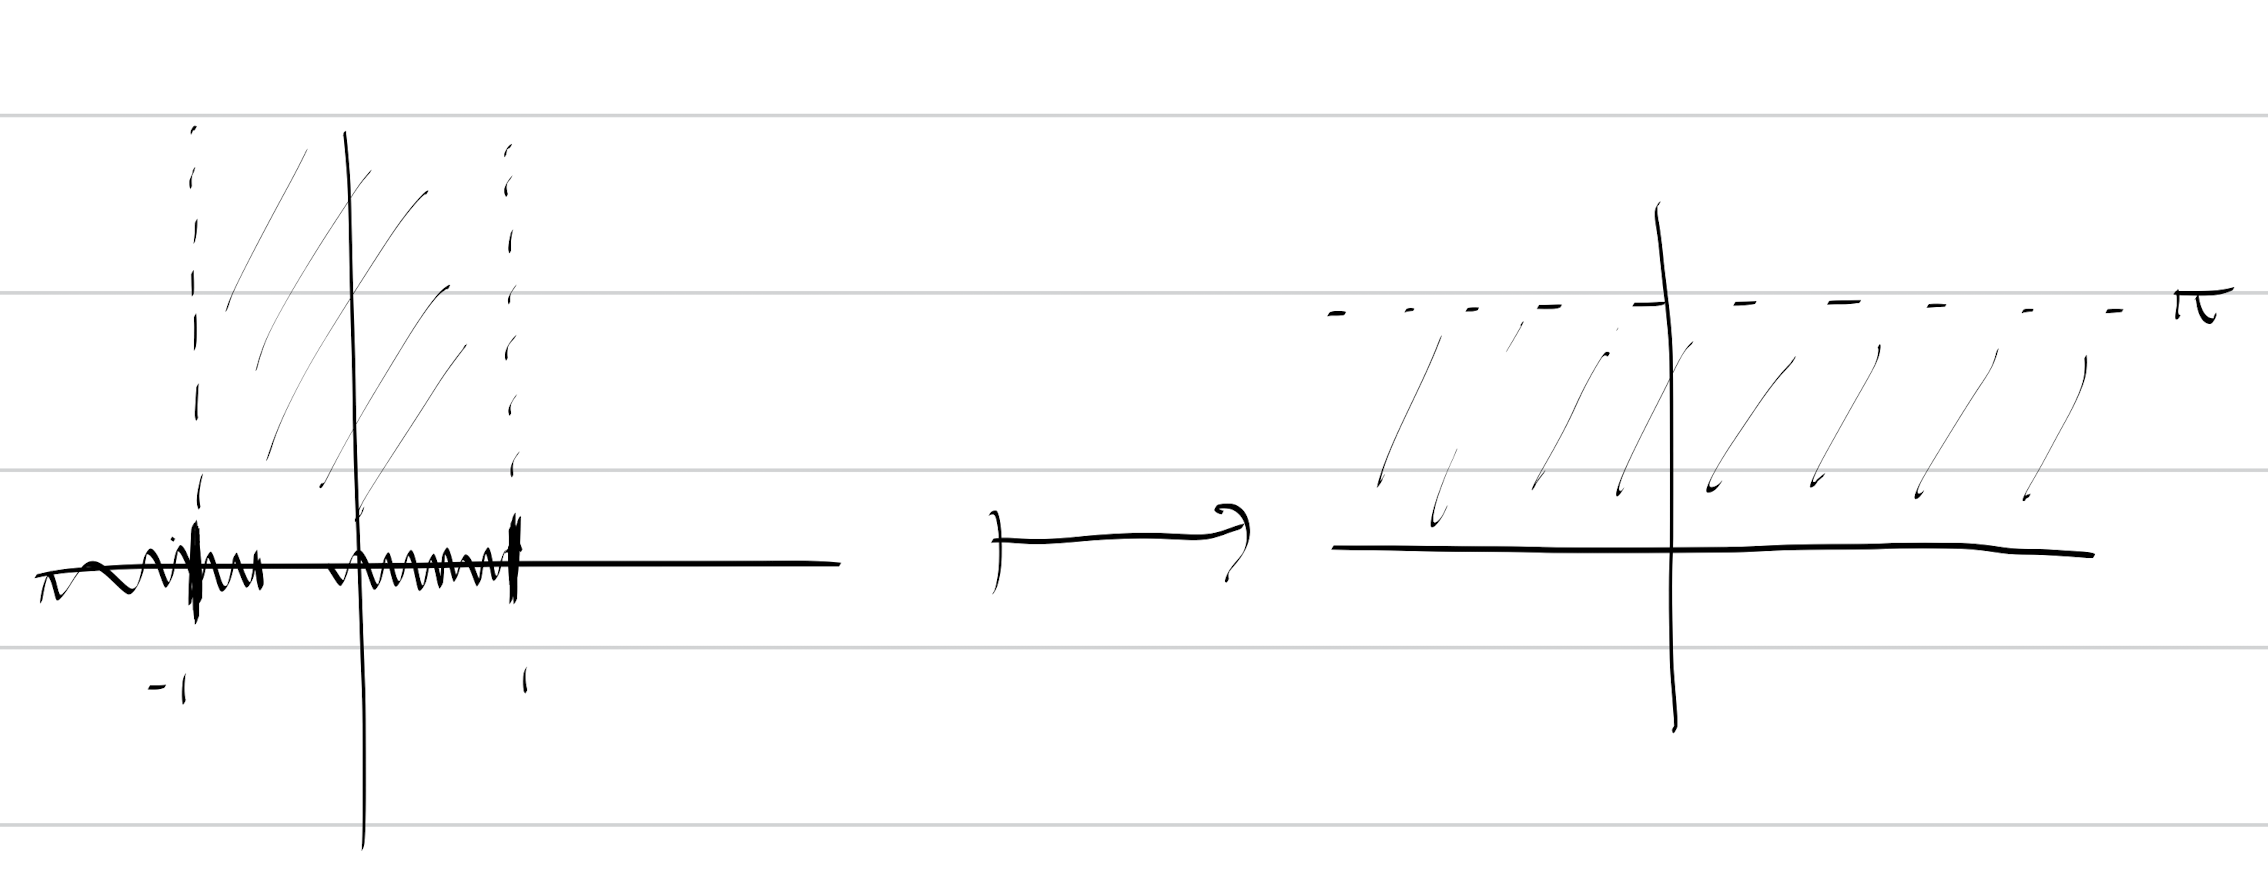
\includegraphics[width=10cm]{images/20_11_c.png}
      \end{center}
  \end{enumerate}
\end{solution}
\begin{solution}[20.12]
  We know that the strip $0 < y < \pi$ maps to the UHP under $w_1 = e^z$. Then, using either the cross ratio or the result in Example 20.3, we use the ratio $\frac{z-i}{z+i}$ to map the UHP into the unit disk. Thus, we have the final conformal map of 
  \begin{align*}
    w(z) &= \frac{e^{z}- i}{e^{z} + i}.
  \end{align*}
  \begin{center}
    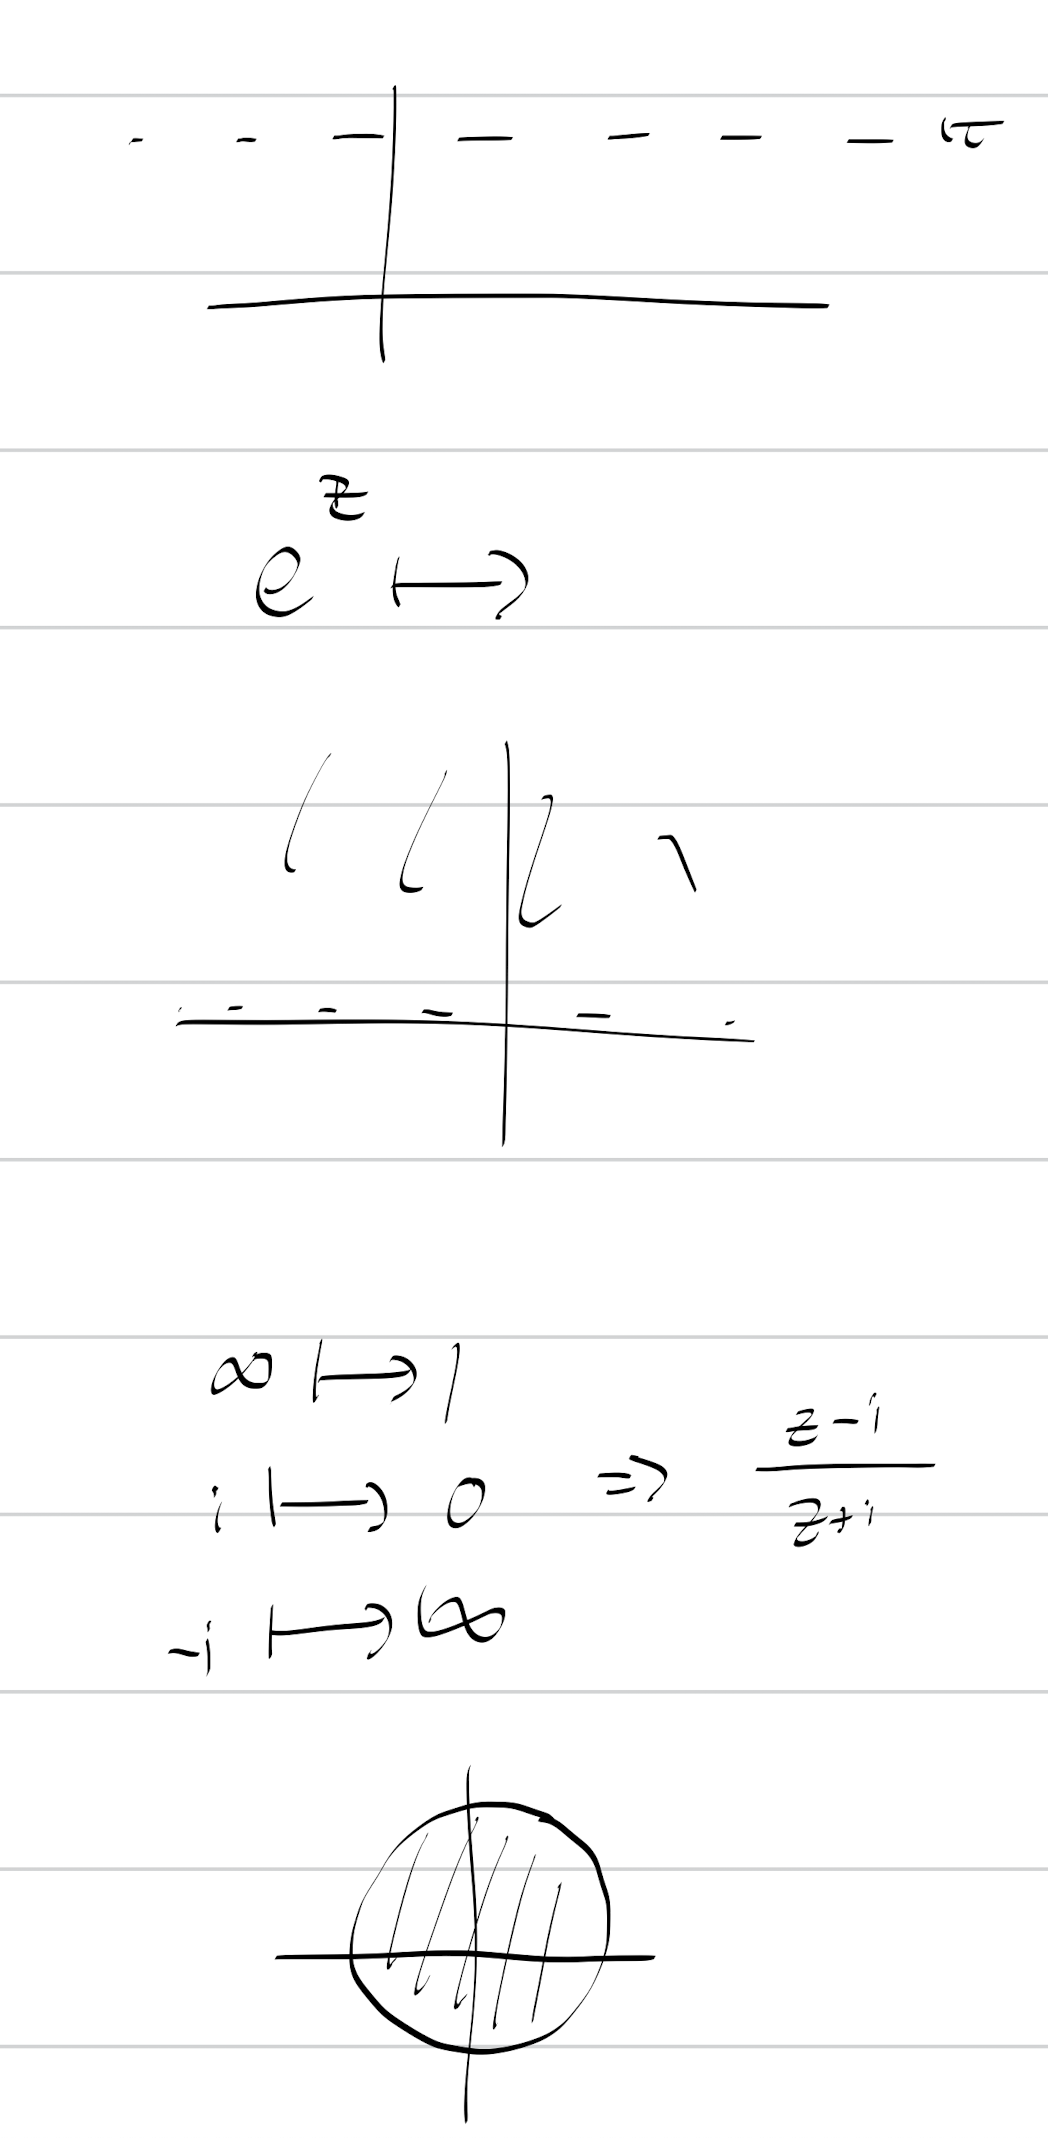
\includegraphics[width=7cm]{images/20_12.png}
  \end{center}
\end{solution}
\begin{solution}[20.14]
  Note that if $z = e^{i\varphi}$ for $0 \leq \varphi \leq \pi$, then
  \begin{align*}
    z + \frac{1}{z} &= e^{i\varphi} + e^{-i\varphi},
  \end{align*}
  which ranges from $-2$ to $2$. Now, if $|x| > 1$, then
  \begin{align*}
    w\left( z \right) &= x + \frac{x}{x^2 + y^2} + i \left( y - \frac{y}{x^2 + y^2} \right),
  \end{align*}
  and, setting $y = 0$, we have
  \begin{align*}
    w(x) &= x + \frac{1}{x}.
  \end{align*}
  This gives a map from the $x$ axis to the $x$ axis.
\end{solution}
\begin{solution}[20.15]
  Taking the derivative of $\Omega$, we get
  \begin{align*}
    \diff{\Omega}{z} &= -iV_0,
  \end{align*}
  with magnitude $\left\vert \diff{\Omega}{z} \right\vert = V_0$.\newline

  I don't know where to go from here (a lack of physics background here is really hurting me here).
\end{solution}
\begin{solution}[20.16]\hfill
  \begin{enumerate}[(a)]
    \item Substituting $z = x + iy$, we get
      \begin{align*}
        w(z) &= \left( x + e^{x}\cos(y) \right) + i \left( y + e^{x}\sin(y) \right)\\
             &= u + iv.
      \end{align*}
      Now, for $y = \pm \pi$, we have that $u < -1$, and that $v = \pm \pi$. The line $y = 0$ maps to $y = 0$.
    \item I'm not sure I exactly understand how to solve for the equipotentials or the electric field lines (or if I've already solved for them?).
  \end{enumerate}
\end{solution}
\begin{solution}[20.17]
  I presume the idea goes something along the lines of the following:
  \begin{enumerate}[(1)]
    \item find a conformal map from the scenario from this scenario to the scenario with two parallel plates (i.e., one conformal map converting the right angles into semi-infinite plates, then the inverse of 20.16);
    \item solving for the electric field/equipotentials in the simpler scenario;
    \item converting back to this scenario.
  \end{enumerate}
  Unfortunately, an issue I am facing here is that I do not know how to do step (1) (or step (3) for that matter).
\end{solution}
\end{document}
